\section{Implementation and Experiments}

\subsection{Experimental Methodology}

In this section we empirically evaluate the CCVPN design paying special attention to the metrics that were earlier discussed in Sec.~\ref{sec:analysis}, i.e., processing overhead, network throughput, and state consumption. In our evaluation we consider the two versions of CCVPN: public key version, and symmetric key version. We here recall that the symmetric key version relies on the assumption that a secure key agreement protocol is performed between the domain's gateways prior to the CCVPN protocol execution.

Our testbed network consists of a butterfly topology, in which the consumers' side and the producers' side gateways are directly interconnected. $N$ producers are connected to the producers' domain gateway and $M$ consumers are connected to the consumers' domain gateway (see Fig.~\ref{create_figure}).

To investigate the processing overhead we measure the average time demand for computing the interests' encapsulation (in public and symmetric key versions), interest decapsulation, content encryption, and content decryption for different content packet sizes (1024, 4096, 16384, and 65536 bytes). We also measure the state consumption for these same four functions.

To compute the overall network throughput we measure the average data-rate for transmissions of 1 to 1,000,000 different interests issues per consumer. We also vary the number of consumers and producers from 1 to 10 of each. Finally, in addition to the network throughput, we also exhibit the total transmission delay for each of the experiments.

\subsection{Results}

\todo{TODO: Add results discussion}

\begin{table}[!h]
\centering
\caption{Interest encapsulation processing times}
\label{my-label}
\begin{tabular}{|l|l|l|l|l|}
\hline
Encapsulation mode   & Encapsulation & Decapsulation \\ \hline
Public Key  & 444$\mu s$           & 449$\mu s$           \\ \hline \cline{4-5} 
Symmetric Key & TODO          & TODO          \\ \hline
\end{tabular}
\end{table}



\begin{table}[!h]
\centering
\caption{Content encryption and decryption times for different payload sizes}
\label{my-label}
\begin{tabular}{|l|l|l|}
\hline
Packet size        & Encryption & Decryption \\ \hline
$1024$B & 125$\mu s$        & 193$\mu s$        \\ \hline
$4096$B & 141$\mu s$        & 220$\mu s$        \\ \hline
$16384$B & 220$\mu s$        & 367$\mu s$        \\ \hline
$65536$B & 519$\mu s$        & 702$\mu s$        \\ \hline
\end{tabular}
\end{table}

\begin{figure}[!t]
\centering
  \subfigure[1 Consumer x 1 Producer]{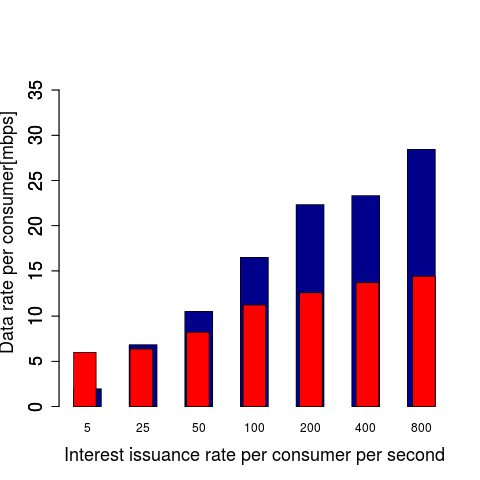
\includegraphics[width=1.5in]{images/throughput_1_1.png}\label{1a}}
  \hfil
  \subfigure[2 Consumers x 1 Producer]{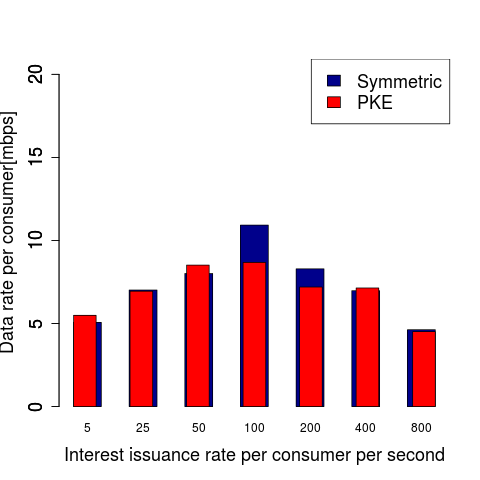
\includegraphics[width=1.5in]{images/throughput_2_1.png}\label{1b}}
  \hfil
  \subfigure[3 Consumers x 1 Producer]{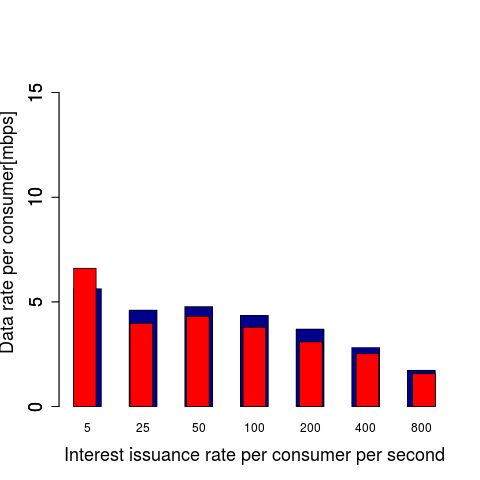
\includegraphics[width=1.5in]{images/throughput_3_1.png}\label{1c}}
  \hfil
  \subfigure[4 Consumers x 1 Producer]{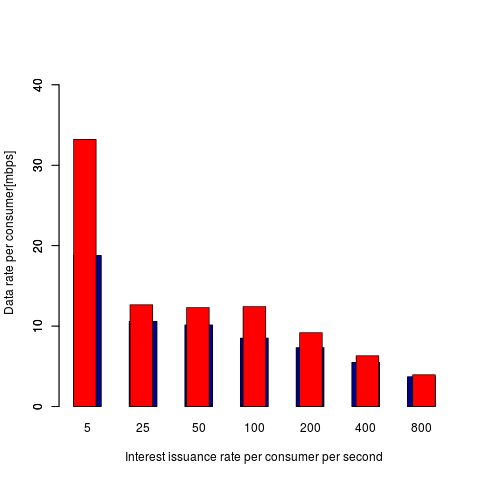
\includegraphics[width=1.5in]{images/throughput_4_1.png}\label{1d}}
\caption{Throughput per consumer. 1 Producer X N consumers. Content packet size: 1024B}\label{exp1}
\end{figure}


\begin{figure}[!t]
\centering
  \subfigure[1 Consumer x 1 Producer]{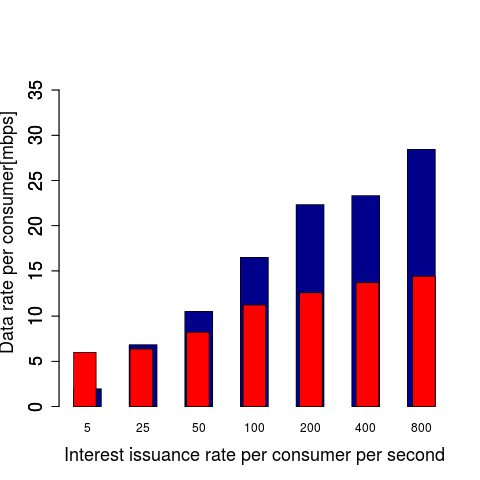
\includegraphics[width=1.5in]{images/throughput_1_1.png}\label{4a}}
  \hfil
  \subfigure[2 Consumers x 2 Producers]{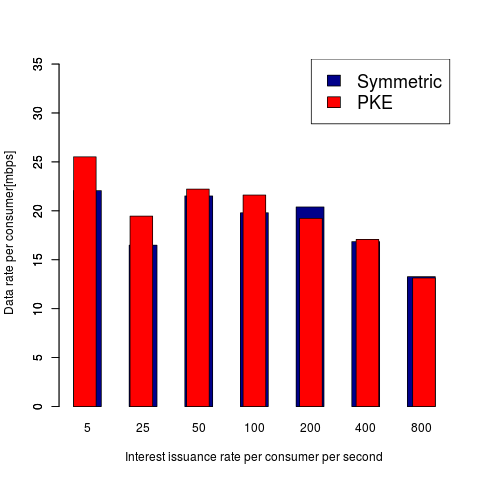
\includegraphics[width=1.5in]{images/throughput_2_2.png}\label{4b}}
  \hfil
  \subfigure[3 Consumers x 3 Producers]{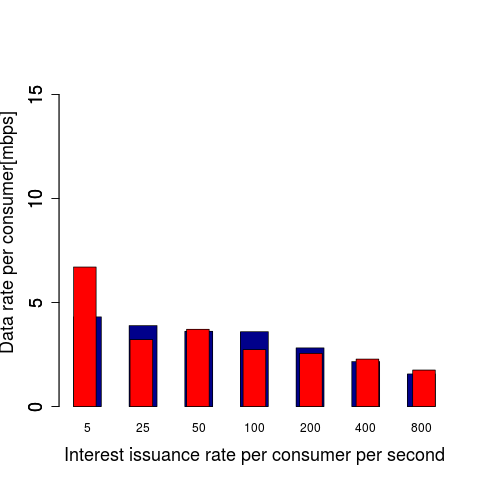
\includegraphics[width=1.5in]{images/throughput_3_3.png}\label{4c}}
  \hfil
  \subfigure[4 Consumers x 4 Producers]{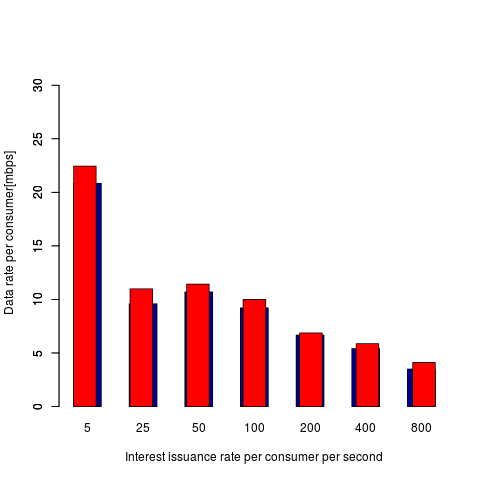
\includegraphics[width=1.5in]{images/throughput_4_4.png}\label{4d}}
\caption{Throughput per consumer. N Producers X N consumers. Content packet size: 1024B}\label{exp4}
\end{figure}


\begin{figure}[!t]
\centering
  \subfigure[1 Consumer x 1 Producer]{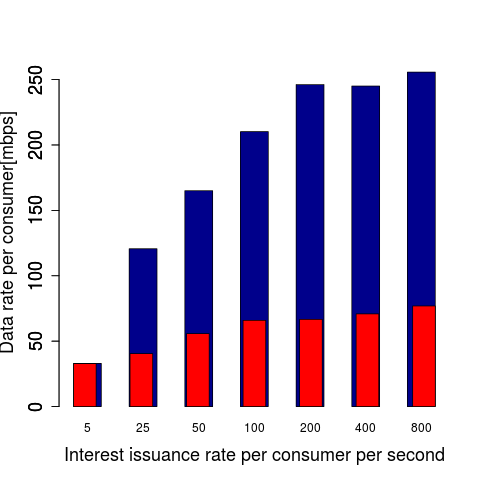
\includegraphics[width=1.5in]{images/10240throughput_1_1.png}\label{1a}}
  \hfil
  \subfigure[2 Consumers x 1 Producer]{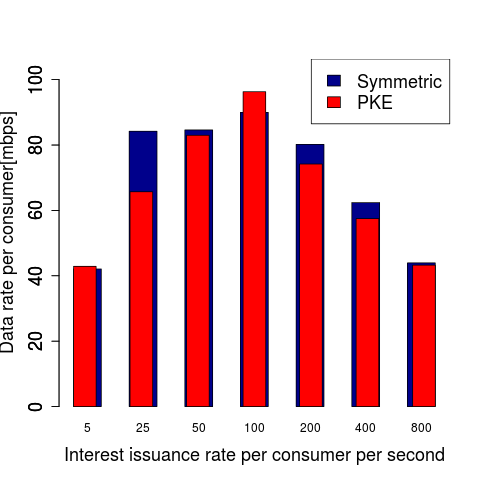
\includegraphics[width=1.5in]{images/10240throughput_2_1.png}\label{1b}}
  \hfil
  \subfigure[3 Consumers x 1 Producer]{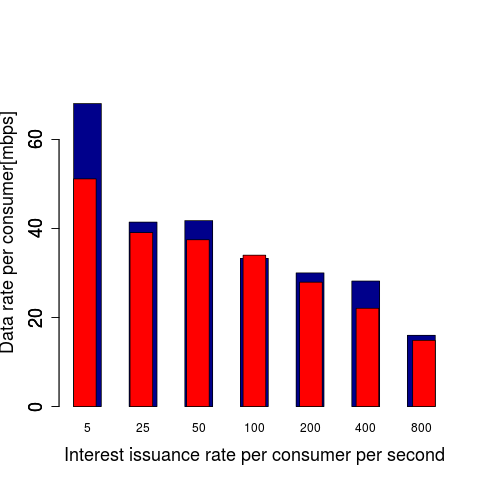
\includegraphics[width=1.5in]{images/10240throughput_3_1.png}\label{1c}}
  \hfil
  \subfigure[4 Consumers x 1 Producer]{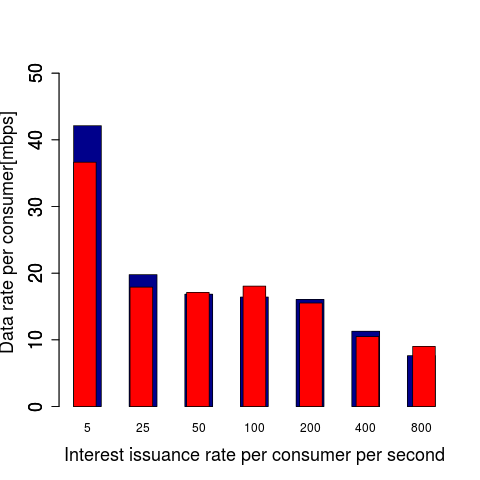
\includegraphics[width=1.5in]{images/10240throughput_4_1.png}\label{1d}}
\caption{Throughput per consumer. 1 Producer X N consumers. Content packet size: 10240B}\label{exp1}
\end{figure}


\begin{figure}[!t]
\centering
  \subfigure[1 Consumer x 1 Producer]{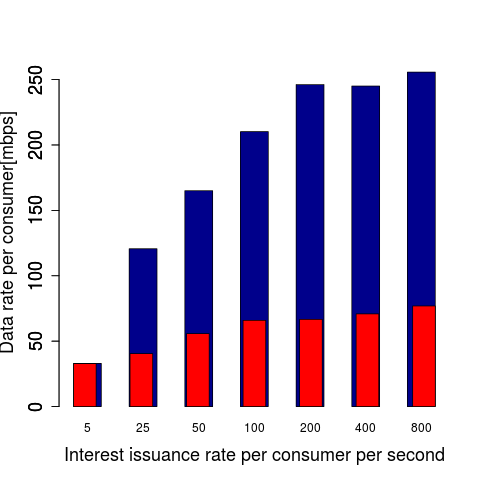
\includegraphics[width=1.5in]{images/10240throughput_1_1.png}\label{4a}}
  \hfil
  \subfigure[2 Consumers x 2 Producers]{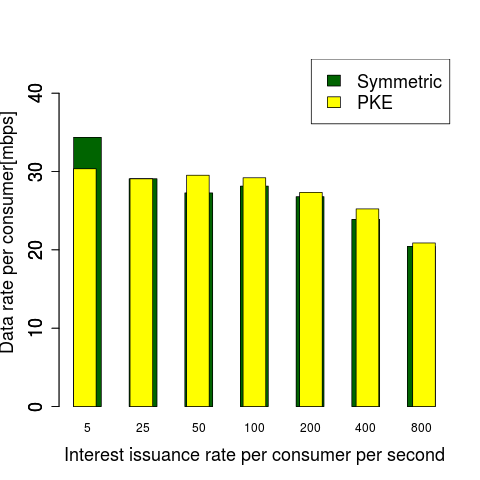
\includegraphics[width=1.5in]{images/10240throughput_2_2.png}\label{4b}}
  \hfil
  \subfigure[3 Consumers x 3 Producers]{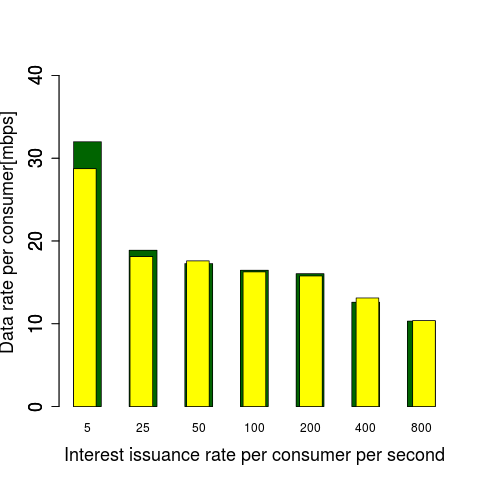
\includegraphics[width=1.5in]{images/10240throughput_3_3.png}\label{4c}}
  \hfil
  \subfigure[4 Consumers x 4 Producers]{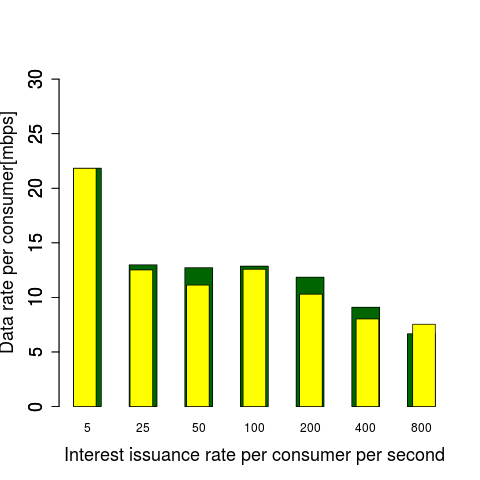
\includegraphics[width=1.5in]{images/10240throughput_4_4.png}\label{4d}}
\caption{Throughput per consumer. N Producers X N consumers. Content packet size: 10240B}\label{exp4}
\end{figure}







\begin{figure}[!t]
\centering
  \subfigure[Throughtput: Content size 1024B]{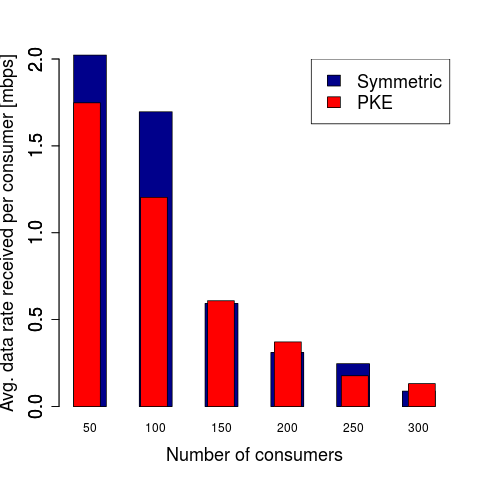
\includegraphics[width=1.5in]{images/1024_many_throughput.png}\label{4a}}
  \hfil
  \subfigure[Dropped packets: Content size 1024B]{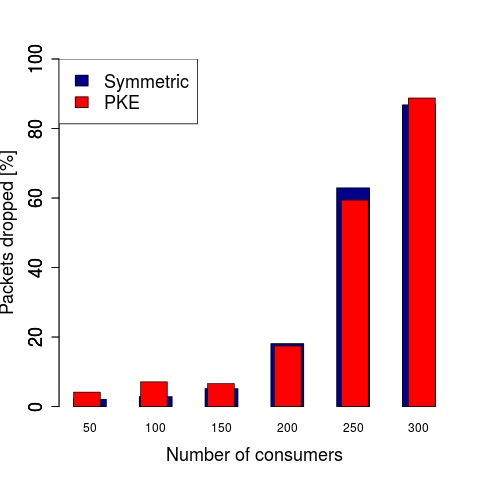
\includegraphics[width=1.5in]{images/1024_many_dropped.png}\label{4b}}
  \hfil
  \subfigure[Throughtput: Content size 10240B]{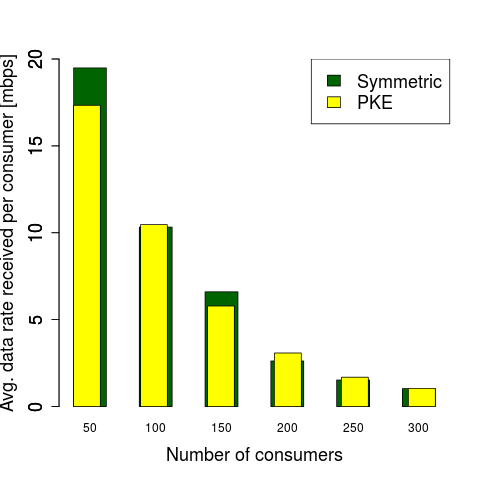
\includegraphics[width=1.5in]{images/10240_many_throughput.png}\label{4c}}
  \hfil
  \subfigure[Dropped packets: Content size 10240B]{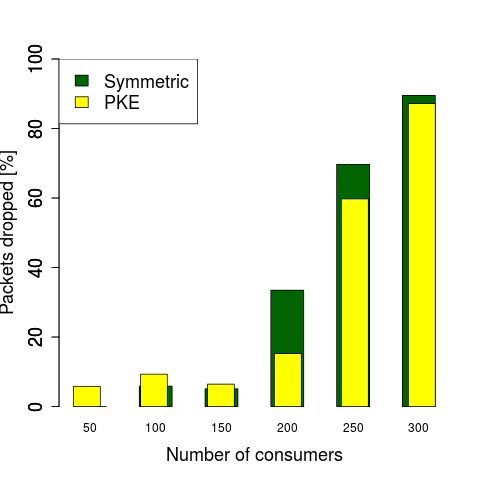
\includegraphics[width=1.5in]{images/10240_many_dropped.png}\label{4d}}
\caption{Throughput per consumer with massive number of consumers/producers. Each consumer issues 5 interests}\label{exp4}
\end{figure}


